\section{Doménový model}
V předchozí podkapitole byla představena MVC architektura a byly popsány její jednotlivé vrstvy. V této bude detailněji přiblížena vrstva modelů a bude již konkrétně představeno, s jakými daty bude aplikace pracovat. Pro znázornění jednotlivých entit včetně jejich důležitých atributů a vztahů mezi nimi je využit doménový model, který je na obrázku \ref{figure:domain-model}. Doménový model byl rozšířen i o datové typy atributů entit a příznak, zda musí být pro daný atribut povinně evidovaná jeho hodnota. Takto povinné atributy entit jsou v modelu označeny symbolem $ \star $.

\begin{landscape}
    \begin{figure}[h]
        \caption{Doménový model}
        \label{figure:domain-model}
        \centering
        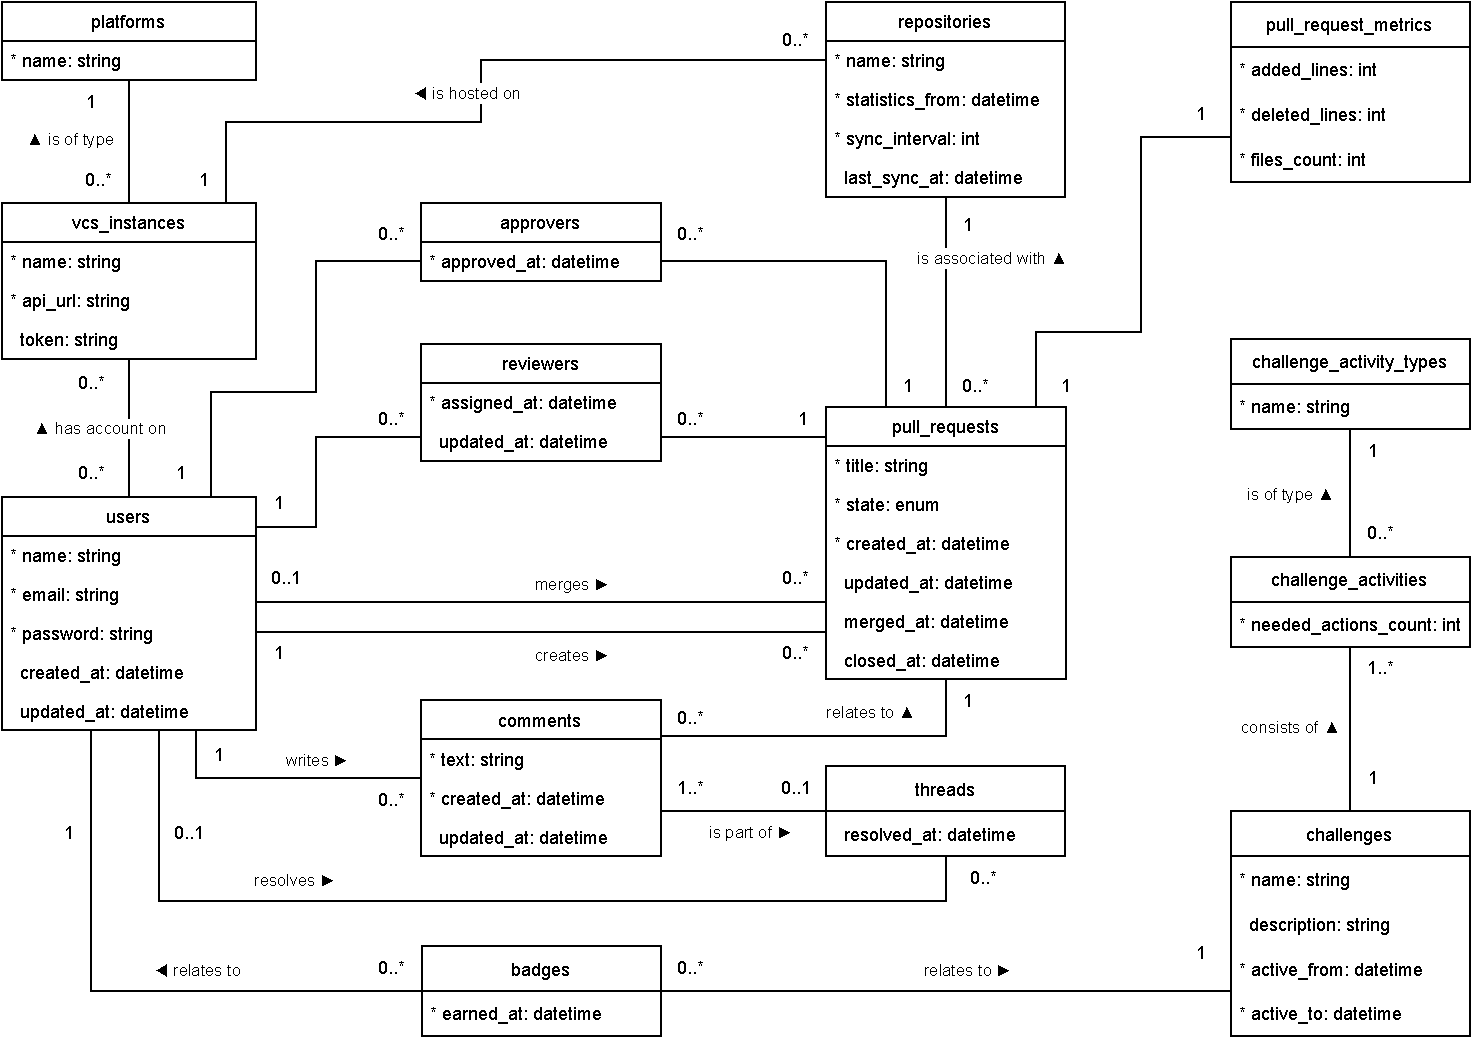
\includegraphics[height=\textheight]{images/domain-model.pdf}
    \end{figure}
\end{landscape}
